\documentclass[12pt,a5paper]{article}
\usepackage[a5paper,margin=6mm]{geometry}
\usepackage{graphicx,subcaption}
\usepackage{amsmath,amsfonts,defns}
\usepackage{pgfplots}
\usepackage[T1]{fontenc}
\usepackage{frcursive}
\usepackage[scr=boondoxo]{mathalfa}

\newcommand{\setfont}[2]{{\fontfamily{#1}\selectfont #2}}
\newcommand{\fcurs}[1]{\text{\setfont{frc}{#1}}}
\newcommand{\bcurs}[1]{\text{$\mathscr{#1}$}}

\newcommand{\Bb}[1]{%
  \expandafter\def\csname#1#1\endcsname%
  {\ensuremath{\mathbb #1}}}
\Bb X\Bb T\Bb R\Bb I\Bb J

\usepackage{pdfcomment}
\newcommand{\ajr}[1]{%
  \pdfcomment[author=AJR,color={1 1 0},subject={#1}]{#1}}
\newcommand{\gaj}[1]{%
  \pdfcomment[author=GAJ,color={0 1 1},subject={#1}]{#1}}
%\renewcommand\Re{\operatorname{\mathfrak{Re}}}
%\renewcommand\Im{\operatorname{\mathfrak{Im}}}

\AtBeginDocument{\listofpdfcomments}

\title{Notes on the Diffusion Equation}
\author{G. Jarrad and A. Roberts}

\begin{document}
\maketitle
\numberwithin{equation}{section}
\numberwithin{figure}{section}
\numberwithin{table}{section}
\section{Introduction}\label{sec:intro}
Consider an arbitrary solution $u:\XX\times \TT\mapsto \RR$ to the simple diffusion equation 
\begin{eqnarray}
	\D tu = \DD xu\,.
	\label{eq:diff}
\end{eqnarray}
A computationally feasible approach would be to 
first establish a sequence  of discrete grid-points,
${\vec X}=[X_j]_{j\in\JJ}$, and thence
summarise the continuum dynamics $u$ by the coarse dynamics
${\vec U}=[U_j]_{j\in\JJ}$, where $U_j(t):=u(X_j,t)$ for all $t\in \TT$.
We may suppose  that ${\vec U}$ evolves temporally according to some self-contained system
\begin{eqnarray}
	\dot{\vec U}(t) = {\vec g}({\vec U}(t))\,.
	\label{eq:temporal}
\end{eqnarray}
Consequently, a link from the coarse dynamics ${\vec U}$ back to the continuum dynamics $u$ might be provided
by choosing an appropriate spatial mapping of the form
\begin{eqnarray}
	u  := u(x,{\vec U}(t)).
	\label{eq:spatial}
\end{eqnarray}
Under this scheme, the linear diffusion equation~(\ref{eq:diff}) becomes
\begin{eqnarray}
	\D {\vec U}{u}\cdot{\vec g} = \DD x{u}\,.
	\label{eq:diff2}
\end{eqnarray}
Observe that the evolution of $u$ now has nonlinear interactions with ${\vec U}$.

\section{Centre Manifold Approximation}\label{sec:centre-man}
The original diffusion equation~(\ref{eq:diff}) admits 
eigensolutions of the form
\begin{eqnarray}
	\tilde{u}(x,t)  = e^{\lambda t+ikx}\,,
\label{eq:raw-eigmode}
\end{eqnarray}
which are physically realisable for real eigenvalues $\lambda=-k^2\le 0$ for 
corresponding eigenmode wavenumbers $\pm k$. 
As a consequence, the transient solutions corresponding
to $\lambda<0$ decay to the centre manifold corresponding to $\lambda=0$. 

This centre manifold can be found in practice by iteratively refining approximations to $u$. In particular, consider a series expansion of the form
\begin{eqnarray}
	u  & \sim & \hat{u}_0+\gamma\hat{u}_1+\gamma^2\hat{u}_2+\cdots\,,
\label{eq:u:series}
\end{eqnarray}
for some parameter $0\le\gamma\le 1$.
Now, the constant eigensolution for $\lambda=0$ implies a slow evolution for the coarse dynamics given by 
equation~(\ref{eq:temporal}), which therefore admits a series expansion of the form
\begin{eqnarray}
	\dot{{\vec U}} & \sim & \gamma {\vec g}_1+\gamma^2 {\vec g}_2+\cdots\,.
\label{eq:Udot:series}
\end{eqnarray}
Hence, equation~(\ref{eq:diff2}) may be decomposed at each order 
$\ell$ of the parameter $\gamma$, giving
\begin{eqnarray}
   \DD {x}{\hat{u}_0} & = & 0\,, \label{eq:pert1}
\\
  \DD {x}{\hat{u}_\ell} & = & \sum_{m=0}^{\ell-1}\D {\vec U}{\hat{u}_m}\cdot{\vec g}_{\ell-m}\,,
\hspace*{5mm}\mbox{for }\ell=1,2,\ldots\,.
\label{eq:pert_ell}
\end{eqnarray}


\section{Leading Approximation}
The leading equation~(\ref{eq:pert1}) admits any spatially piecewise linear function as a solution. 
Hence, in keeping
with the discretisation imposed by the coarse dynamics of Section~\ref{sec:intro},
let the spatial domain be partitioned into contiguous intervals, namely $\XX=\bigcup_{j\in\JJ^+}\II_j$, where
$\II_j:=[X_{j-1},X_j]$ and $\JJ^+:=\JJ\backslash\{\underline{J}\}$ with $\underline{J}:=\inf\JJ$.
Then, consider the piecewise  linear approximation
\begin{eqnarray}
   \hat{u}_0 = \sum_{j\in\JJ^+}\chi_j(\xi_j U_j+(1-\xi_j)U_{j-1})\,,
\label{eq:uhat0}
\end{eqnarray}
with indicator $\chi_j(x)=1$ (or 0) for $x\in\II_j$ (or $x\not\in\II_j$), and linear interpolator
$\xi_j(x)=\frac{x-X_{j-1}}{X_j-X_{j-1}}$.
This particular approximation is chosen to be continuous across the 
internal interval boundaries,
namely $X_j=\II_j\bigcap\II_{j+1}$ for $j\in\JJ^0:=\JJ^+\backslash\{\bar{J}\}$, where $\bar{J}:=\sup\JJ$. 
In general, it suffices 
to impose a continuity condition at the right-hand end of each interval, namely:
\begin{eqnarray}
   [u]_j = 0 && \forall j\in\JJ^0\,,
\label{eq:cont-cond}
\end{eqnarray}
where $ [u]_j := \lim_{\epsilon\rightarrow 0^{+}} u(X_j+\epsilon,t)-u(X_j-\epsilon,t)$.
Unfortunately, this linear approximation is not smooth at the interval boundaries. 
For convenience, consider regular grid spacings of size 
$X_j-X_{j-1}=H$. Then, denoting $\D xu$ as $u'$, observe that
\begin{eqnarray}
   [\hat{u}'_0]_j = \frac{1}{H}(U_{j+1}+U_{j-1}-2U_j)~=~\frac{1}{H}\left.\delta^{2}\hat{u}_0\right|_{X_j}\,,
\end{eqnarray}
for the centred difference $\delta u(x,t):= u(x+\frac{H}{2},t)-u(x-\frac{H}{2},t)$\,.
However, this non-smoothness may be corrected at higher order by imposing a further internal boundary condition, namely
\begin{eqnarray}
   [u']_j = \frac{1-\gamma}{H}\left.\delta^{2}u\right|_{X_j}\hspace*{5mm}\forall j\in\JJ^0\,.
\label{eq:smooth-cond}
\end{eqnarray}
Consequently, smooth approximations are found in the limit as $\gamma\rightarrow 1$.

\section{Linear Eigenmode Analysis}\label{sec:eig:modes}
Consider a single eigenmode of the form~(\ref{eq:raw-eigmode}) for some arbitrary, 
non-dimensionalised wavenumber $\kappa:=kH>0$. 
Thus, allowing for the partitioning of \XX, let
\begin{eqnarray}
\tilde{u} & \sim & \sum_{j\in\JJ^+} \chi_j a_j e^{i\kappa\xi_j} + \text{c.c.}\,,
\end{eqnarray}
for arbitrary, time--varying, complex coefficients $a_j=A_j+iB_j$. 
We now seek the `spatial' evolution from interval to interval for the given wavenumber.
The continuity condition~(\ref{eq:cont-cond}) implies that
\begin{eqnarray}
a_{j+1} - a_j e^{i\kappa\xi_j} + \text{c.c.} = 0\,.
\end{eqnarray}
Similarly, the smoothness condition~(\ref{eq:smooth-cond}) implies that 
\begin{eqnarray}
i\kappa a_{j+1} -i\kappa a_j e^{i\kappa} + \text{c.c.} =  
(1-\gamma)\left(
a_{j+1} e^{i\kappa} + a_j - 2 a_j e^{i\kappa}
\right)
+ \text{c.c.}\,,
\end{eqnarray}
where continuity has also been invoked at the left-hand of the $j$th interval.
In coefficient form, the update from the $j$th to $(j+1)$th segment is
\begin{eqnarray}
\left[\begin{array}{cc}
1 & 0\\
\bcurs{f}\bcurs{c} & 1-\bcurs{f}\fcurs{s}\\
\end{array}\right]
\left[\begin{array}{c}
A_{j+1}\\
B_{j+1}\\
\end{array}\right]
=
\left[\begin{array}{cc}
\bcurs{c} & -\fcurs{s}\\
\fcurs{s}+f(2\bcurs{c}-1) & \bcurs{c}-2\bcurs{f}\fcurs{s}\\
\end{array}\right]
\left[\begin{array}{c}
A_{j}\\
B_{j}\\
\end{array}\right]\,,
\end{eqnarray}
where $\bcurs{c}+i\fcurs{s}:=e^{i\kappa}$ and $\bcurs{f}:=(1-\gamma)/\kappa$.
Now, letting $a_{j+1}=\mu a_j$, the characteristic equation for 
the growth factor $\mu$ is
\begin{eqnarray}
(1-\bcurs{f}\fcurs{s})\left[\mu^2-2\frac{\bcurs{c}-\bcurs{f}\fcurs{s}}{1-\bcurs{f}\fcurs{s}}\mu+1\right] = 0\,,
\end{eqnarray}
with roots given by
\begin{eqnarray}
\mu & = & \beta\pm\sqrt{\beta^2-1}
\hspace*{5mm}\mbox{for } 
\beta~=~\frac{\bcurs{c}-\bcurs{f}\fcurs{s}}{1-\bcurs{f}\fcurs{s}}\,.
\end{eqnarray}
Observe that $\beta\le 1$ since $\bcurs{c}=\cos\kappa\le 1$ and 
$1-\bcurs{f}\fcurs{s}=1-(1-\gamma)\frac{\sin\kappa}{\kappa}\ge 0$.
Thus, for $|\beta|<1$, the factors are complex with magnitude 
$|\mu|=1$,
indicating marginally stable evolution of $a_j$. 
This includes the limiting case of $\gamma=1$ ($f=0$), for which
$\mu=\bcurs{c}\pm i\fcurs{s}=e^{\pm i\kappa}$.
Likewise, $\mu=\pm 1$ for $\beta=\pm 1$, corresponding to $\kappa=n\pi$, $n=0,1,2,\ldots$.
Finally, for small regions near each $\kappa=(2n+1)\pi$, 
it is found that $\beta<-1$, resulting in two real factors,
$\mu<-1$ and $-1<\mu<0$, indicating unstable (saddle) evolution.
More precisely, these unstable regions occur when
\begin{eqnarray}
%c-fs < -(1-fs) & \Rightarrow & 1+c < 2fs 
%\frac{kH}{1-\gamma}\cos^2\frac{kH}{2} < 2\sin\frac{kH}{2}\cos\frac{kH}{2}\,.
\frac{\kappa}{2} <(1-\gamma)\tan\frac{\kappa}{2}\,, && \kappa\ne n\pi\,.
\label{eq:leaforbid}
\end{eqnarray}
Thus, at equilibrium ($\gamma=0$) there is an initial forbidden gap $\kappa\in(0,\pi)$ adjacent to the centre manifold
wavenumber $\kappa=0$ (see Figure~\ref{fig:leaspec}), indicating that transient solutions decay to the centre manifold at a rate of at least
$\lambda=-k^2=-\frac{\pi^2}{H^2}$. It is this gap that provides robustness to nonlinear perturbations
of the system about the equilibrium.

\begin{figure}[hbt]
\centering
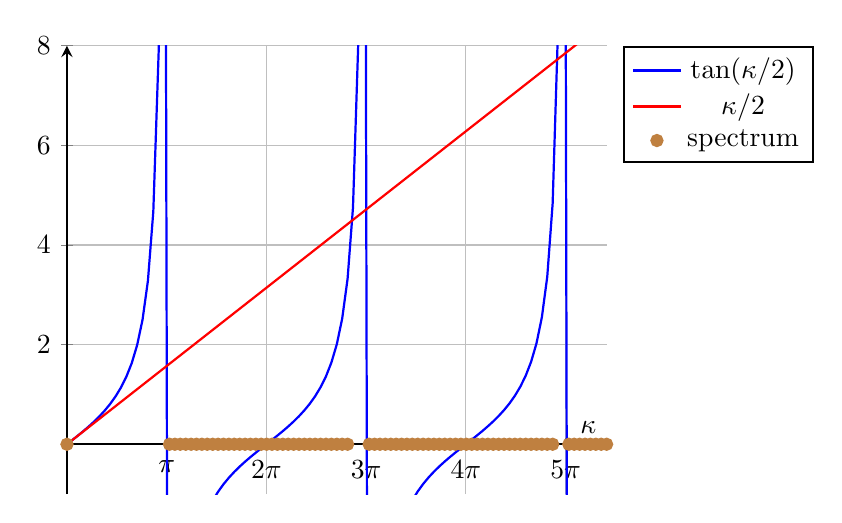
\begin{tikzpicture}
\begin{axis}[ xlabel={$\kappa$}
  ,axis x line=middle,axis y line=middle
  ,thick,grid,samples=101
  ,ymin=-1,ymax=8 ,domain=0:17
  ,xtick={3.1416,6.2832,9.4248,12.5664,15.7080}
  ,xticklabels={$\pi$,$2\pi$,$3\pi$,$4\pi$,$5\pi$}
  ,legend pos=outer north east
  ] 
\addplot [blue,no marks] {tan(deg(x)/2)}; 
\addlegendentry{$\tan(\kappa/2)$};
\addplot [red,no marks,samples=2] {x/2}; 
\addlegendentry{$\kappa/2$};
\addplot [brown,only marks,mark=*] {0-99*(x/2<tan(deg(x)/2))};
\addlegendentry{spectrum};
\end{axis}
\end{tikzpicture}
\caption{The equilibrium spectrum determined by the forbidding condition~\eqref{eq:leaforbid}.}
\label{fig:leaspec}
\end{figure}


\section{Linear Dual Space}
Assume for convenience that there are at least $|\JJ|\ge 3$ discrete grid-points, and thus $|\JJ^+|\ge 2$ intervals.
Then an appropriate inner product for spatially square-integrable fields $u$ and $v$ is given by
\begin{eqnarray}
\langle u,v\rangle = \int_{X_{\underline{J}}}^{X_{\bar{J}}}uv\;dx
= \sum_{j\in\JJ^+}\int_{\II_j}uv\;dx := \sum_{j\in\JJ^+}{\cal I}_j uv\,.
\label{eq:inner}
\end{eqnarray}
It can then be shown, for twice-differentiable fields, that
\begin{eqnarray}
\langle u'',v\rangle =
\langle u,v''\rangle + R\,,
\end{eqnarray}
with residual 
\begin{eqnarray}
R &= & \sum_{j\in\JJ^+}[r]_{X_{j-1}}^{X_j}
= r_{\bar{J}}-r_{\underline{J}}-\sum_{j\in\JJ^0}[r]_j\,,
\end{eqnarray}
for $r=u'v-v'u$.
Now, assuming that both $u$ and $v$ obey conditions~(\ref{eq:cont-cond}) and~(\ref{eq:smooth-cond}), 
the residual jump at $X_j$ becomes
\begin{eqnarray}
[r]_j & = & [u']_j V_j-[v']_j U_j
\nonumber\\
& = & \frac{1-\gamma}{H}\left[
(U_{j+1}+U_{j-1})V_j-(V_{j+1}+V_{j-1})U_j
\right]\,.
\end{eqnarray}
Observe that terms from surrounding intervals $\II_{j-1}$ and $\II_{j+1}$ will cancel terms from $\II_j$, leaving
only contributions from the outermost boundary intervals $\II_{\underline{J}+1}$ and $\II_{\bar{J}}$; consequently:
\begin{eqnarray}
R & = & 
u'_{\bar{J}}V_{\bar{J}}-v'_{\bar{J}}U_{\bar{J}}
-u'_{\underline{J}}V_{\underline{J}}+v'_{\underline{J}}U_{\underline{J}}
\nonumber\\ &&
{}-\frac{1-\gamma}{H}\left[
U_{\bar{J}}V_{\bar{J}-1}-V_{\bar{J}}U_{\bar{J}-1}
+U_{\underline{J}}V_{\underline{J}+1}-V_{\underline{J}}U_{\underline{J}+1}
\right]\,.
\end{eqnarray}
On a finite domain, there are three main outer boundary conditions that lead to a zero residual:
\begin{description}
\item[periodic] Having period $\bar{J}-\underline{J}$ corresponds to \(U_{\bar{J}}=U_{\underline{J}}\). Furthermore, by joining
the domain cylindrically at $X_{\underline{J}}$ and $X_{\bar{J}}$,  it can be shown that
\begin{eqnarray}
u'_{\underline{J}}-u'_{\bar{J}} = [u']_{\bar{J}} = \frac{1-\gamma}{H}(U_{\underline{J}+1}+U_{\bar{J}-1}-2U_{\bar{J}})\,,
\end{eqnarray}
using condition~\eqref{eq:smooth-cond}. Hence, $R=0$ if correspondingly $v$ is periodic with period $\bar{J}-\underline{J}$.
\item[Dirichlet] Setting \(u=0\) at the boundaries corresponds to \(U_{\underline{J}}=U_{\bar{J}}=0\), 
giving $R=0$ if correspondingly \(v=0\) on the boundaries.
\item[Neumann] Requiring \(u'=0\) on the boundaries  (for $\gamma=1$) corresponds to 
\begin{eqnarray}
u'_{\underline{J}}=\frac{1-\gamma}{H}(U_{\underline{J}+1}-U_{\underline{J}})\,,
&&
u'_{\bar{J}}=\frac{1-\gamma}{H}(U_{\bar{J}}-U_{\bar{J}-1})\,,
\end{eqnarray}
giving $R=0$ if correspondingly \(v'=0\) on the boundaries.
\end{description}
Under any of the above three conditions, observe that $\langle{\cal L}u,v\rangle =\langle u,{\cal L}v\rangle$
for ${\cal L}=\DD {x}{}$, and hence ${\cal L}$ is self-adjoint.
Furthermore, we are free to choose any dual $v$, e.g.\ to satisfy ${\cal L}v=0$ for conenience.
In particular, we may specifically target the $j$-th interval for $u$ by selecting $v=\hat{v}_0^{[j]}$, where
\begin{eqnarray}
\hat{v}_0^{[j]} := \chi_j\xi_j + \chi_{j+1}(1-\xi_{j+1})\hspace*{5mm}\forall j\in\JJ^0\,.
\label{eq:vhat0}
\end{eqnarray}
Observe that this dual satisfies conditions~\eqref{eq:cont-cond} and~\eqref{eq:smooth-cond} for $\gamma=0$.
%It can then be shown in general (see Section~\ref{sec:inner}) that
%\begin{eqnarray}
%\langle u'', \hat{v}_0^{[j]}\rangle = -[u']_j+\frac{1}{H}\left.\delta^2 u\right|_{X_j}\,,
%\label{eq:udd:vhat0}
%\end{eqnarray}
%for any continuous, twice-differentiable field $u$.

\section{First-order Approximation}\label{sec:first-order}
Substituting the leading approximation~(\ref{eq:uhat0}) into the
nonlinear diffusion equation~(\ref{eq:pert_ell}) for $\ell=1$ results in
the first-order equation
\begin{eqnarray}
\hat{u}''_1 = \sum_{j\in\JJ^+}\chi_j(\xi_j g_{1,j}+(1-\xi_j)g_{1,j-1})\,.
\label{eq:uhat:1:dd}
\end{eqnarray}
Spatial integration then gives
\begin{eqnarray}
\hat{u}'_1 & = & \frac{H}{2}\sum_{j\in\JJ^+}\chi_j(\xi^2_j g_{1,j}
-(1-\xi_j)^2g_{1,j-1}+c_{1,j})\,,
\label{eq:udhat1}
\\
\hat{u}_1 & = & \frac{H^2}{6}\sum_{j\in\JJ^+}\chi_j(\xi^3_j g_{1,j}
+(1-\xi_j)^3g_{1,j-1}+3\xi_{j}c_{1,j}+d_{1,j})\,.
\label{eq:uhat1}
\end{eqnarray}
Recall from the chosen  spatial discretisation that $u|_{X_j}=U_{j}$ at each grid-point.
Observe this is already satified by $\hat{u}_0$ from equation~(\ref{eq:uhat0}), implying
from expansion~(\ref{eq:u:series}) that
\begin{eqnarray}
\left.\hat{u}_\ell\right|_{X_j}\equiv 0 && \mbox{for }\ell=1,2,\ldots\,.
\label{eq:u_ell_fixed}
\end{eqnarray}
Thus $[\hat{u}_\ell]_j=0$, satisfying the continuity 
condition~(\ref{eq:cont-cond}), and furthermore $\delta^2\hat{u}_\ell|_{X_j}=0$.
Now, evaluating equation~(\ref{eq:uhat1}) at $\xi_j=0$ gives $d_{1,j}=-g_{1,j-1}$,
and at $\xi_j=1$ gives $3c_{1,j}=-(g_{1,j}-g_{1,j-1})$.
Thus,  from equation~(\ref{eq:udhat1}), observe that
\begin{eqnarray}
[\hat{u}'_1]_j = -H\left(1+\frac{1}{6}\delta^2\right)g_{1,j}\,.
\end{eqnarray}
However, the smoothness condition~(\ref{eq:smooth-cond}) gives
\begin{eqnarray}
   [\hat{u}'_1]_j = 
\frac{1}{H}\left.\delta^{2}\hat{u}_1\right|_{X_j}
-\frac{1}{H}\left.\delta^{2}\hat{u}_0\right|_{X_j}
= -\frac{1}{H}\delta^{2}U_j\,,
\label{eq:udhat1-jump}
\end{eqnarray}
and hence
\begin{eqnarray}
\left(1+\frac{1}{6}\delta^2\right)g_{1,j} = \frac{1}{H^2}\delta^2U_j\,.
\label{eq:g1}
\end{eqnarray}
This solution can also be otained more directly via the dual space by computing $\langle\hat{u}''_1,\hat{v}_0^{[j]}\rangle$ from
equations~\eqref{eq:vhat0} and~\eqref{eq:uhat:1:dd}, and using results~\eqref{eq:udd:vhat0} and~\eqref{eq:udhat1-jump}.
Consequently, as a first approximation, the coarse dynamics evolve according to
\begin{eqnarray}
	\dot{\vec U} = \frac{\gamma}{H^2}S\delta^2\vec U + {\cal O}(\gamma^2)\,,
\label{eq:Udot:1}
\end{eqnarray}
from equations~\eqref{eq:temporal} and~\eqref{eq:Udot:series},
where, for convenience, we define the non-local operator $S:=(1+\frac{1}{6}\delta^2)^{-1}$.

Now, recall that Section~\ref{sec:eig:modes} introduced the non-dimensionalised wavenumber $\kappa:=kH$. 
For convenience, we here likewise define a non-dimensionalised expansion rate of $\bar{\lambda}:=\lambda H^2$.
Hence, the eigensolution~\eqref{eq:raw-eigmode} may be rewritten as $\tilde{u}(x,t)=e^{\bar{\lambda}t/H^2+i\kappa x/H}$, 
such that the spectrum of equation~\eqref{eq:diff} becomes $\bar{\lambda}=-\kappa^2$.
It can further be shown that
$\delta^2\tilde{u}=-2(1-\bcurs{c})\tilde{u}$, where, as before, $\bcurs{c}=\cos\kappa$. 
Hence, the spectrum of the first-order approximation (with $\gamma=1$) is given by
\begin{eqnarray}
\bar{\lambda} = -\frac{6(1-\bcurs{c})}{(2+\bcurs{c})} \sim -\kappa^2-\frac{1}{12}\kappa^4+{\cal O}(\kappa^6)\,,
\label{eq:spec:1st}
\end{eqnarray}
which reveals an error of size ${\cal O}(\kappa^4)$ in comparison to the exact spectrum.

The stability of the approximate dynamics is shown by Figures~\ref{fig:spec:first-order:nd}--\ref{fig:spec:first-order}.
Observe that the turning point of the approximation occurs at $\kappa=\pi$,
where the continuum eigenmode becomes
 $\tilde{u}(x,t)=e^{\bar{\lambda}t/H^2+i\pi x/H}$.
This gives rise\footnote{Since $X_j=X_0+jH$, and the neglected coefficient is arbitrary.} 
to a sawtooth mode in the coarse dynamics of the form $\tilde{U}_j=e^{\bar{\lambda}t/H^2}(-1)^{j}$.
Hence, from either equation~\eqref{eq:spec:1st} with $\bcurs{c}=\cos\pi=-1$, or from 
 equation~\eqref{eq:Udot:1} with $\gamma=1$ and $\delta^2\tilde{U}_j=-4\tilde{U}_j$,
we obtain $\bar{\lambda}=-12$, in contrast to the true value of
$\bar{\lambda}=-\pi^2$, giving an error of $\Delta\bar{\lambda}\approx-2.1$.
%Using the right-hand side of  equation~\eqref{eq:spec:1st} instead leads to an approximate error estimate of
%$\Delta\bar{\lambda}\approx-\frac{\pi^4}{12H^2}\approx-\frac{8.1}{H^2}$.
%% \cos kH \sim 1-k^2H^2/2+k^4H^4/24-O(k^6H^6).
%% -2(1-\cos kH) \sim -k^2H^2+k^4H^4/12-...
%% 1/(2+\cos kH) \sim 1/3(1-k^2H^2/6+...) = (1/3)*(1+k^2H^2/6-...)
%% -6(1-\cos kH)/(2+\cos kH) \sim (-k^2H^2+k^4H^4/12+...)*(1+k^2H^2/6+...)  = -k^2H^2-k^4H^4/6+k^2H^2/12+...
%%  = -k^2H^2-k^4H^4/12+...
\begin{figure}[hbt]
\centering
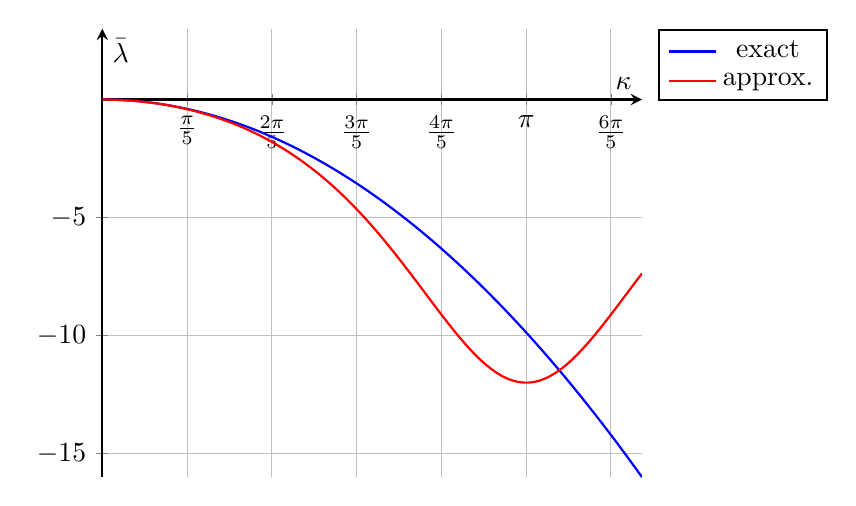
\begin{tikzpicture}
\begin{axis}[ xlabel={$\kappa$}, ylabel={$\bar{\lambda}$}
  ,axis x line=middle,axis y line=middle
  ,thick,grid,no marks,samples=101
  ,domain=0:4,ymax=3
  ,xtick={0.62832,1.25664,1.88496,2.51328,3.1416,3.76992}
  ,xticklabels={$\frac{\pi}{5}$,$\frac{2\pi}{5}$,$\frac{3\pi}{5}$,$\frac{4\pi}{5}$,$\pi$,$\frac{6\pi}{5}$}
  ,legend pos=outer north east
  ] 
\addplot  {0-(x^2)}; 
\addlegendentry{exact};
\addplot {-6*(1-cos(deg(x)))/(2+cos(deg(x)))}; 
\addlegendentry{approx.};
\end{axis}
\end{tikzpicture}
\caption{The  non-dimensionalised spectrum ($\bar{\lambda}$ versus~$\kappa$) of the linear diffusion equation, contrasting the 
continuum dynamics against the discrete, first-order approximation (for $\gamma=1$).}
\label{fig:spec:first-order:nd}
\end{figure}

\begin{figure}[hbt]
\centering
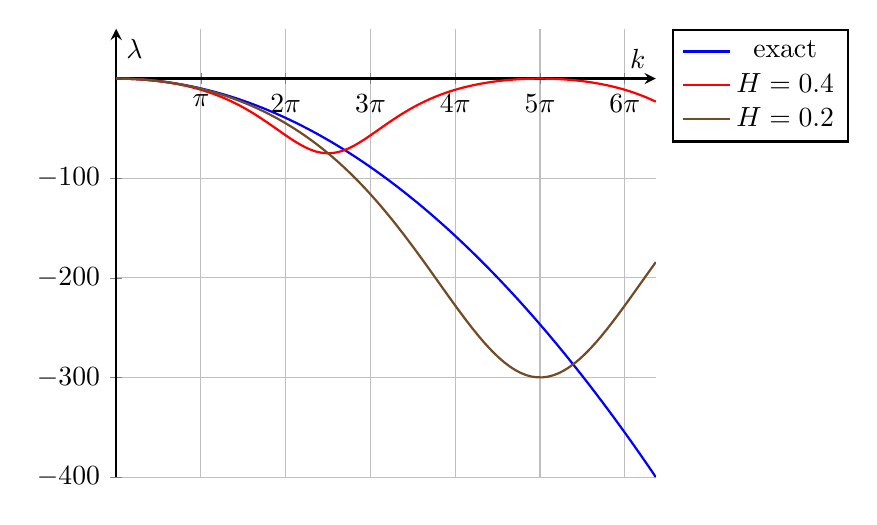
\begin{tikzpicture}
\begin{axis}[ xlabel={$k$}, ylabel={$\lambda$}
  ,axis x line=middle,axis y line=middle
  ,thick,grid,no marks,samples=101
  ,domain=0:20,ymax=50
  ,xtick={3.1416,6.2832,9.4248,12.5664,15.7080,18.8496}
  ,xticklabels={$\pi$,$2\pi$,$3\pi$,$4\pi$,$5\pi$,$6\pi$}
  ,legend pos=outer north east
  ] 
\addplot  {0-(x^2)}; 
\addlegendentry{exact};
\addplot {-6/0.4^2*(1-cos(deg(x*0.4)))/(2+cos(deg(x*0.4)))}; 
\addlegendentry{$H=0.4$};
\addplot {-6/0.2^2*(1-cos(deg(x*0.2)))/(2+cos(deg(x*0.2)))}; 
\addlegendentry{$H=0.2$};
\end{axis}
\end{tikzpicture}
%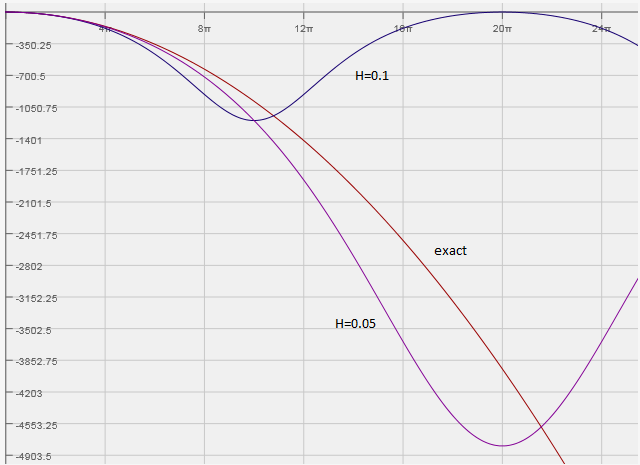
\includegraphics[width=0.8\textwidth]{figures/first-order-spectrum.png}
\caption{The  dimensionalised spectrum ($\lambda$ versus~$k$) of the linear diffusion equation, contrasting the 
continuum dynamics against the discrete, first-order approximation (for $\gamma=1$) with interval length $H$.}
\label{fig:spec:first-order}
\end{figure}

\section{Second-order Approximation}
For convenience, consider the right--shift operator $\sigma u(x,t) := u(x+H,t)$;
 whence $\delta:=\sigma^{{1}/{2}}-\sigma^{-{1}/{2}}$.
Then, from equation~\eqref{eq:pert_ell} for $\ell=2$, we obtain
\begin{eqnarray}
  \hat{u}''_2 & = & \D{\vec U}{\hat{u}_0}\cdot{\vec g}_{2}+\D{\vec U}{\hat{u}_1}\cdot{\vec g}_{1}
\nonumber\\
& = & \sum_{j\in\JJ^+}\chi_j\left\{\xi_j+(1-\xi_j)\sigma^{-1}\right\}g_{2,j}
\nonumber\\
&& {}-\frac{1}{6}\sum_{j\in\JJ^+}\chi_j\xi_j(1-\xi_j)\left\{
(2-\xi_j)\sigma^{-1}+(1+\xi_j)
\right\}S\delta^2g_{1,j}\,,
\label{eq:uhat2:dd}
\end{eqnarray}
using equations~\eqref{eq:uhat0} , \eqref{eq:uhat1}, and~\eqref{eq:g1}.
Next, observe 
from equations~\eqref{eq:udd:vhat0}, \eqref{eq:smooth-cond} and \eqref{eq:u_ell_fixed} that
\begin{eqnarray}
\langle\hat{u}''_\ell,\hat{v}_0^{[j]}\rangle\equiv0 && \mbox{for }\ell=2,3,\ldots\,.
\end{eqnarray}
Alternatively, it can be shown by direct integration and simplification that
\begin{eqnarray}
\langle\hat{u}''_2,\hat{v}_0^{[j]}\rangle = HS^{-1}g_{2,j}-\frac{H}{6}\left(\frac{7}{60}\delta^2+\frac{1}{2}\right)S\delta^2g_{1,j}\,,
\end{eqnarray}
from equations~\eqref{eq:vhat0} and~\eqref{eq:uhat2:dd}.
Hence, as a second approximation, the coarse dynamics evolve according to
\begin{eqnarray}
	\dot{\vec U} = \frac{\gamma}{H^2}S\delta^2\vec U 
+ \frac{\gamma^2}{60H^2}(7-2S)S^2\delta^4\vec U
+ {\cal O}(\gamma^3)\,,
\end{eqnarray}
using the fact that $S\delta^2=6(1-S)$.
%%on div; off allfac; factor h,k,gamma;
%%let k^8 => 0;
%%c:=1-k^2H^2/2+k^4*H^4/24-k^6*h^6/720;
%%Dsq:=-2*(1-c); Si:=1+Dsq/6;
%%S:=1-(Si-1)+(Si-1)^2-(Si-1)^3;
%%lam:=gamma*S*Dsq/H^2+gamma^2*(7-2*S)*S^2*Dsq^2/(60*H^2);
%%lam -> -k^2+H^4*k^6/180+O(H^6k^8)

Thus, following Section~\ref{sec:first-order}, the approximate spectrum (for $\gamma=1$) is now
\begin{eqnarray}
\bar{\lambda} = -\frac{3(1-\bcurs{c})(32+41\bcurs{c}+17\bcurs{c}^2)}{5(2+\bcurs{c})^3}
\sim -\kappa^2-\frac{1}{180}\kappa^6+{\cal O}(\kappa^8)\,.
\end{eqnarray}
Observe that the ${\cal O}(\kappa^4)$ error term from the first-order approximation~\eqref{eq:spec:1st} has now been
completely eliminated by the second-order correction, in favour of an ${\cal O}(\kappa^6)$ error. 
This adjusted spectral behaviour is shown in Figure~\ref{fig:spec:2nd-order:nd}.
Observe that the turning point again occurs at $\kappa=\pi$. Hence,
as per Section~\ref{sec:first-order},
the sawtooth mode (with $\bcurs{c}=-1$) now has a decay rate of $\bar{\lambda}=-9.6$, leading to an error of
$\Delta\bar{\lambda}\approx 0.27$, which is an order of magnitude smaller than the first-order error.
%% \cos kH \sim 1-k^2H^2/2+k^4H^4/24-O(k^6H^6).
%% -2(1-\cos kH) \sim -k^2H^2+k^4H^4/12-...
%% 1/(2+\cos kH) \sim 1/3(1-k^2H^2/6+...) = (1/3)*(1+k^2H^2/6-...)
%% -6(1-\cos kH)/(2+\cos kH) \sim (-k^2H^2+k^4H^4/12+...)*(1+k^2H^2/6+...)  = -k^2H^2-k^4H^4/6+k^2H^2/12+...
%%  = -k^2H^2-k^4H^4/12+...
%\begin{figure}[hbt]
%\centering
%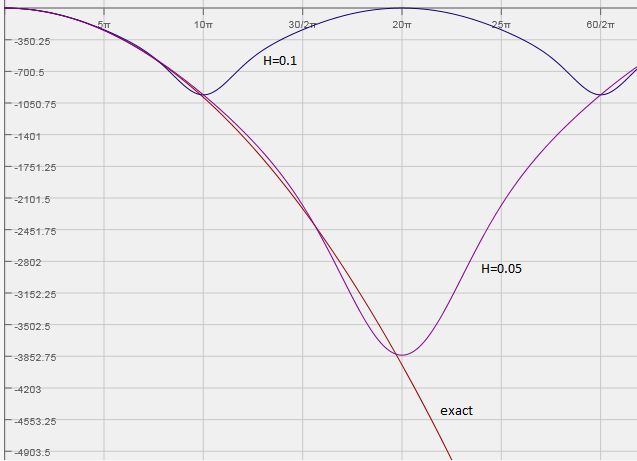
\includegraphics[width=0.8\textwidth]{figures/second-order-spectrum.png}
%\begin{tikzpicture}
%\begin{axis}[ xlabel={$k$}, ylabel={$\lambda$}
% ,axis x line=middle,axis y line=middle
% ,thick,grid,no marks,samples=101
% ,domain=0:20,ymax=50
% ,xtick={3.1416,6.2832,9.4248,12.5664,15.7080,18.8496}
% ,xticklabels={$\pi$,$2\pi$,$3\pi$,$4\pi$,$5\pi$,$6\pi$}
% ,legend pos=outer north east
% ] 
%\addplot  {0-(x^2)}; 
%\addlegendentry{exact};
%\addplot %{-1/5/0.4^2*(96+27*cos(deg(x*0.4))-72*cos(deg(x*0.4))^2-51*cos(deg(x*0.4))^3)/(8+12*cos(deg(x*0.4))+6*cos(deg(x*0.4))^2+cos(deg(x*0.4))^3)}; 
%\addlegendentry{$H=0.4$};
%\addplot %{-1/5/0.2^2*(96+27*cos(deg(x*0.2))-72*cos(deg(x*0.2))^2-51*cos(deg(x*0.2))^3)/(8+12*cos(deg(x*0.2))+6*cos(deg(x*0.2))^2+cos(deg(x*0.2))^3)}; 
%\addlegendentry{$H=0.2$};
%\end{axis}
%\end{tikzpicture}
%\caption{The exact spectrum ($\lambda$ versus $k$) of the linear diffusion equation, compared to a second-order approximation with $H=0.4$ %and $H=0.2$ for $\gamma=1$.}
%\label{fig:spec:2nd-order}
%\end{figure}
\begin{figure}[hbt]
\centering
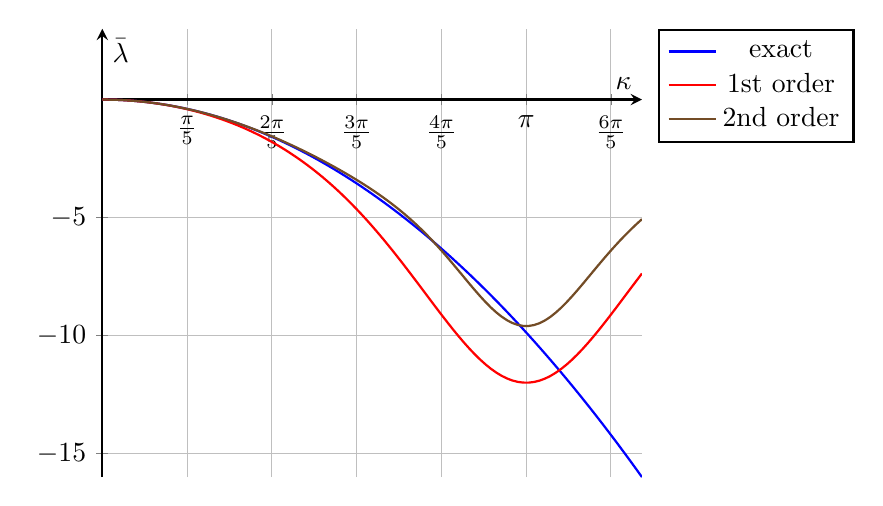
\begin{tikzpicture}
\begin{axis}[ xlabel={$\kappa$}, ylabel={$\bar{\lambda}$}
  ,axis x line=middle,axis y line=middle
  ,thick,grid,no marks,samples=101
  ,domain=0:4,ymax=3
  ,xtick={0.62832,1.25664,1.88496,2.51328,3.1416,3.76992}
  ,xticklabels={$\frac{\pi}{5}$,$\frac{2\pi}{5}$,$\frac{3\pi}{5}$,$\frac{4\pi}{5}$,$\pi$,$\frac{6\pi}{5}$}
  ,legend pos=outer north east
  ] 
\addplot  {0-(x^2)}; 
\addlegendentry{exact};
\addplot {-6*(1-cos(deg(x)))/(2+cos(deg(x)))}; 
\addlegendentry{1st order};
\addplot {-1/5*(96+27*cos(deg(x))-72*cos(deg(x))^2-51*cos(deg(x))^3)/(8+12*cos(deg(x))+6*cos(deg(x))^2+cos(deg(x))^3)}; 
\addlegendentry{2nd order};
\end{axis}
\end{tikzpicture}
\caption{The  non-dimensionalised spectrum ($\bar{\lambda}$ versus~$\kappa$) of the linear diffusion equation, contrasting the 
continuum dynamics against the first two discrete approximations (for $\gamma=1$).}
\label{fig:spec:2nd-order:nd}
\end{figure}

\section{Linear Advection}\label{sec:lin-adv}
The addition of linear advection of speed $C$ to the diffusion equation~\eqref{eq:diff} leads to the
linear diffusion--advection equation
\begin{eqnarray}
	\D tu = \DD xu - C\D xu\,.
	\label{eq:diff-adv}
\end{eqnarray}
Now, recalling that ${\cal L}=\DD{x}{}$ and $\vec{g}=\dot{\vec{U}}$, let equation~\eqref{eq:diff-adv} be rewritten in the form
\begin{eqnarray}
{\cal M}(u,g) & := & {\cal L}u-C\D xu-\D{\vec{U}}{u}\cdot\vec{g}~=~0\,.
\label{eq:Mug}
\end{eqnarray}
Under the assumption that $u$ still obeys the continuity condition~\eqref{eq:cont-cond} and the smoothness condition~\eqref{eq:smooth-cond}, this equation may in turn be transformed\footnote{Via the inner product of terms with the
linear dual solution $\hat{v}_0^{[j]}$, from equation~\eqref{eq:vhat0}.} into the solvability condition
\begin{eqnarray}
       {\cal S}(u,g) & := & 
          \frac{\gamma}{H}\delta^2u|_{X_j} - \frac{C}{H}(\sigma-1){\cal I}_j u
	-{\cal I}_j\left(\D {\vec U}u\hat{v}_0^{[j]}\right)\cdot\vec{g}~=~0 \,,
\label{eq:Sug}
\end{eqnarray}
where ${\cal I}_j u := \int_{\II_j}u\,dx$
from equation~\eqref{eq:inner}, and
use has been made of results~\eqref{eq:udd:vhat0} and~\eqref{eq:ud:vhat0}.

Next, recall the initial continuum approximation of $u\approx\hat{u}_0$, from equation~\eqref{eq:uhat0},
with the corresponding coarse evolution of $\hat{\vec{g}}\approx\hat{\vec{g}}_0=\vec{0}$. Observe that this
`solution' approximately satisfies equations~\eqref{eq:Mug} and~\eqref{eq:Sug}, since
${\cal M}(\hat{u}_0,\hat{\vec{g}}_0)={\cal O}(\gamma+C)$ and
${\cal S}(\hat{u}_0,\hat{\vec{g}}_0)={\cal O}(\gamma+C)$.
This suggests a two-step approach to refining the approximation: firstly, find a correction
$\hat{\vec{g}}_1$ to $\hat{\vec{g}}_0$ such that ${\cal S}(\hat{u}_0,\hat{\vec{g}}_0+\hat{\vec{g}}_1)={\cal O}(\gamma^{2}+C^{2})$;
and, secondly, find a correction
$\hat{u}_1$ to $\hat{u}_0$ such that ${\cal M}(\hat{u}_0+\hat{u}_1,\hat{\vec{g}}_0+\hat{\vec{g}}_1)={\cal O}(\gamma^{n+1}+C^{n+1})$.
In general, let\footnote{Now using an implicit dependence 
upon $\gamma$ and $C$, in contrast to the explicit dependence assumed in expansions~\eqref{eq:u:series} and~\eqref{eq:Udot:series}.} 
\begin{eqnarray}
u & \sim & \hat{u}_0+\hat{u}_1+\hat{u}_2+\cdots\,,
\label{eq:new:u:series}
\\
\vec{g} & \sim & \hat{\vec{g}}_0+\hat{\vec{g}}_1+\hat{\vec{g}}_2+\cdots\,,
\label{eq:new:g:series}
\end{eqnarray}
where\footnote{Alternative schemes will differ in the definition of $\hat{u}_n$  and $\hat{\vec{g}}_n$.} 
$\hat{u}_n=\sum_{p,q|p+q=n}a_{p,q}\gamma^p C^q$, and similarly for $\hat{\vec{g}}_n$. 
Then, it can be shown that substitution of these expansions into the solvability condition~\eqref{eq:Sug} gives
\begin{eqnarray}
{\cal I}_j\left(\D {\vec U}{u_0}\hat{v}_0^{[j]}\right)\cdot\vec{g}_n & = &
{\cal S}(\hat{u}_0+\cdots+\hat{u}_{n-1},
\hat{\vec{g}}_0+\cdots+\hat{\vec{g}}_{n-1})
\nonumber\\
&&{}+{\cal O}(\gamma^{n+1}+C^{n+1})\,.
\label{eq:Sug:n}
\end{eqnarray}
Similarly, substitution of the expansions into the manifold equation~\eqref{eq:Mug} leads to
\begin{eqnarray}
{\cal L}\hat{u}_n & = & -{\cal M}(\hat{u}_0+\cdots+\hat{u}_{n-1},
\hat{\vec{g}}_0+\cdots+\hat{\vec{g}}_{n-1})
\nonumber\\
&&{}+\D{\vec{U}}{\hat{u}_0}\cdot\hat{\vec{g}}_n+O(\gamma^{n+1}+C^{n+1})\,.
\end{eqnarray}
For example, for $n=1$ the solvability condition~\eqref{eq:Sug:n} reduces to
\begin{eqnarray}
	H\left(1+\frac{1}{6}\delta^2\right)\hat{g}_{1,j} & = & 
\gamma\frac{\delta^2U_j}{H} - C\mu\delta U_j\,,
\end{eqnarray}
where $\mu:=(\sigma^{{1}/{2}}+\sigma^{-{1}/{2}})/2$, whereupon
\begin{eqnarray}
	g_j & = & \dot{U}_j~=~
\gamma S\frac{\delta^2U_j}{H^2} - CS\frac{\mu\delta U_j}{H} + {\cal O}(\gamma^2+C^2)\,,
\end{eqnarray}
Observe that the first and second spatial derivatives in equation~\eqref{eq:diff-adv} are here
approximated by centred differences, which follows
naturally from the derivation. This is in contrast to the usual approach of difference equations,
where the first derivative, for example, could arbitrarily be approximated by a forward, backward or centred difference.

Next,  after finding $\hat{u}_1$ (not shown here), the approximate solution is refined at step $n=2$, giving
\begin{eqnarray}
	\dot{U}_j & = & 
\gamma S\frac{\delta^2U_j}{H^2} - CS\frac{\mu\delta U_j}{H} 
\nonumber\\&&
{}-\frac{\gamma^2}{10}S(S-1)(7-2S)\frac{\delta^2 U_j}{H^2}
-\frac{2\gamma C}{5}S(S-1)^2\frac{\mu\delta U_j}{H}
\nonumber\\&&
{}-\frac{C^2}{20}(S-1)^2(2S-1)U_j+ {\cal O}(\gamma^3+C^3)
\,.
\label{eq:Udot:adv:2}
\end{eqnarray}
Observe that choosing a time-scale of $H^2$, as before, leads naturally to an advection parameterisation in terms of $\bar{C}:=CH$.
The spectrum of equation~\eqref{eq:diff-adv} is then $\bar{\lambda}=-\kappa^2-i\kappa\bar{C}$.
In contrast, the spectrum (for $\gamma=1$) of approximation~\eqref{eq:Udot:adv:2} is given by
\begin{eqnarray}
\Re\bar{\lambda} & = & -\frac{3(1-\bcurs{c})(32+41\bcurs{c}+17\bcurs{c}^2)}{5(2+\bcurs{c})^3}
-\frac{\bar{C}^2}{20}\frac{(1-\bcurs{c})^2(4-\bcurs{c})}{(2+\bcurs{c})^3}\,,
\\
\Im\bar{\lambda} & = & 
-\bar{C}\frac{3\fcurs{s}}{2+\bcurs{c}}\left[1+\frac{2(1-\bcurs{c})^2}{5(2+\bcurs{c})^2}\right]\,,
\end{eqnarray}
recalling that $\bcurs{c}+i\fcurs{s}:=e^{i\kappa}$ and observing that $\mu\delta\tilde{u}=i\fcurs{s}\tilde{u}$.
Some plots of the real and imaginary parts of this spectrum are shown in 
Figures~\ref{fig:spec:adv:re:2nd-order:nd}--\ref{fig:spec:adv:im:2nd-order:nd}.
\begin{figure}[hbt]
\centering
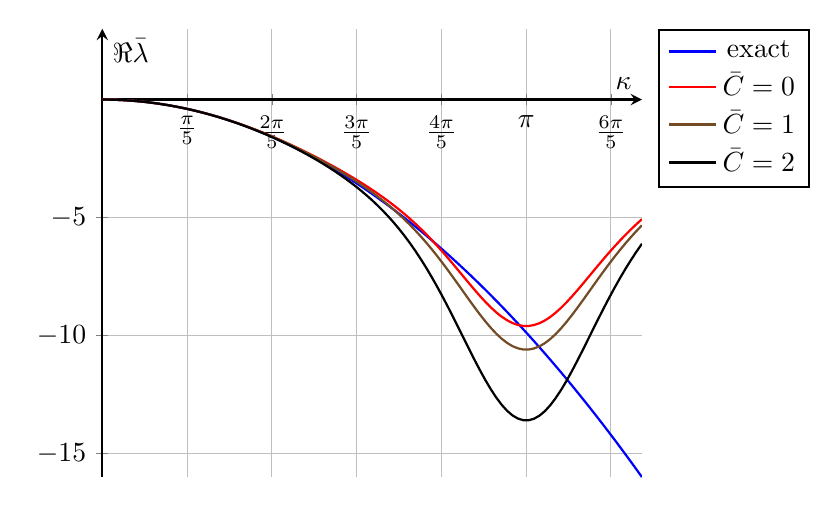
\begin{tikzpicture}
\begin{axis}[ xlabel={$\kappa$}, ylabel={$\Re\bar{\lambda}$}
  ,axis x line=middle,axis y line=middle
  ,thick,grid,no marks,samples=101
  ,domain=0:4,ymax=3
  ,xtick={0.62832,1.25664,1.88496,2.51328,3.1416,3.76992}
  ,xticklabels={$\frac{\pi}{5}$,$\frac{2\pi}{5}$,$\frac{3\pi}{5}$,$\frac{4\pi}{5}$,$\pi$,$\frac{6\pi}{5}$}
  ,legend pos=outer north east
  ] 
\addplot  {0-(x^2)}; 
\addlegendentry{exact};
\addplot {-3/5*(1-cos(deg(x)))*(32+41*cos(deg(x))+17*cos(deg(x))^2)/(2+cos(deg(x)))^3};
\addlegendentry{$\bar{C}=0$};
\addplot {-3/5*(1-cos(deg(x)))*(32+41*cos(deg(x))+17*cos(deg(x))^2)/(2+cos(deg(x)))^3
-1^2/20*(1-cos(deg(x)))^2*(4-cos(deg(x)))/(2+cos(deg(x)))^3};
\addlegendentry{$\bar{C}=1$};
\addplot {-3/5*(1-cos(deg(x)))*(32+41*cos(deg(x))+17*cos(deg(x))^2)/(2+cos(deg(x)))^3
-2^2/20*(1-cos(deg(x)))^2*(4-cos(deg(x)))/(2+cos(deg(x)))^3};
\addlegendentry{$\bar{C}=2$};
\end{axis}
\end{tikzpicture}
\caption{The  real--part of the non-dimensionalised spectrum ($\bar{\lambda}$ versus~$\kappa$) of the linear diffusion--advection equation, contrasting the continuum dynamics against the 2nd-order discrete approximation (for $\gamma=1$), for various
values of non-dimensionalised advection speed $\bar{C}$.}
\label{fig:spec:adv:re:2nd-order:nd}
\end{figure}
\begin{figure}[hbtp]
\centering
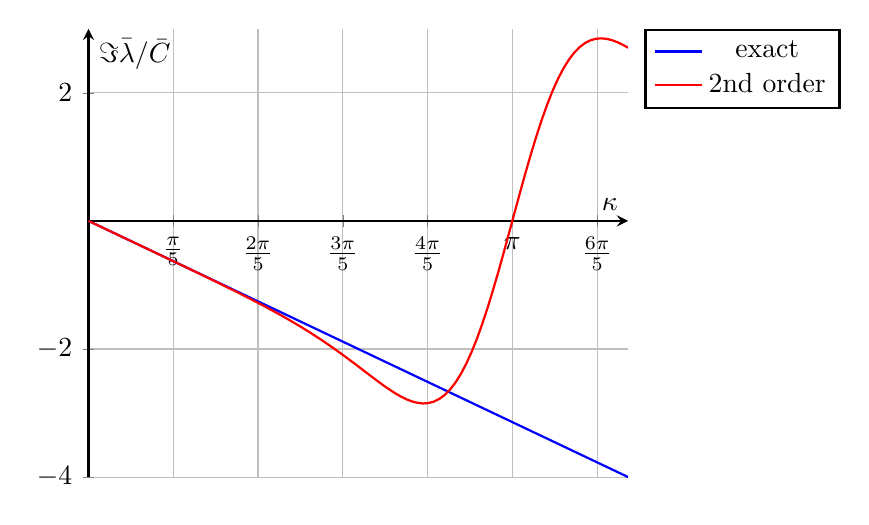
\begin{tikzpicture}
\begin{axis}[ xlabel={$\kappa$}, ylabel={$\Im\bar{\lambda}/\bar{C}$}
  ,axis x line=middle,axis y line=middle
  ,thick,grid,no marks,samples=101
  ,domain=0:4,ymax=3
  ,xtick={0.62832,1.25664,1.88496,2.51328,3.1416,3.76992}
  ,xticklabels={$\frac{\pi}{5}$,$\frac{2\pi}{5}$,$\frac{3\pi}{5}$,$\frac{4\pi}{5}$,$\pi$,$\frac{6\pi}{5}$}
  ,legend pos=outer north east
  ] 
\addplot  {0-(x)}; 
\addlegendentry{exact};
\addplot {-3*sin(deg(x))/(2+cos(deg(x)))*(1+2/5*(1-cos(deg(x)))^2/(2+cos(deg(x)))^2)};
\addlegendentry{2nd order};
\end{axis}
\end{tikzpicture}
\caption{The  imaginary--part of the non-dimensionalised spectrum ($\bar{\lambda}$ versus~$\kappa$) of the linear diffusion--advection equation, contrasting the continuum dynamics against the 2nd-order discrete approximation (for $\gamma=1$).}
\label{fig:spec:adv:im:2nd-order:nd}
\end{figure}

In order to see that the $\bar{C}^2$ term is an artifact of the expansion of $\dot{U}_j$, 
higher order terms in $\gamma$ are first found\footnote{Changing, for computational convenience, to the use of rectangular truncation
${\cal O}(\gamma^n,\bar{C}^3)$, 
in place of the previous circular truncation ${\cal O}(\gamma^3+\bar{C}^3)$.}, and then $S$ is replaced by its asymptotic expansion
\begin{eqnarray}
S & \sim & 1-\frac{1}{6}\delta^2+\frac{1}{36}\delta^4-\frac{1}{216}\delta^6+\frac{1}{1296}\delta^8-\frac{1}{7776}\delta^{10}+\cdots\,.
\end{eqnarray}
The resulting coefficients of the partial sums $\sum_{p=0}^{n}C^2\gamma^p \delta^qU_j$ are summarised in Table~\ref{tab:terms}.
Observe that terms for each fixed $q$ cancel out (at $\gamma=1$) for a sufficiently high truncation order $n$,
indicating that the expansion of the coarse dynamics approximation is consistent with the continuum dynamics.
\begin{table}
\caption{The coefficients of the partial sums $\sum_{p=0}^{n}C^2\gamma^p\delta^q U_j$ in the 
asymptotic expansion of $\hat{g}_j$ for leading values of $n$ and $q$.}
\label{tab:terms}
\centering
\begin{tabular}{cccccc}
\hline
$n\backslash q$ & 4 & 6 & 8 & 10 & 12\\
\hline
&&&&&\\[-2ex]
0 & $-\frac{1}{720}$ & $\frac{1}{1080}$ & $-\frac{1}{2880}$        & $\frac{1}{9720}$            & $-\frac{5}{186624}$\\[1ex]
1 & $\frac{1}{720}$  & $-\frac{1}{945}$  & $\frac{131}{302400}$ & $-\frac{167}{1360800}$ & $\frac{167}{6531840}$\\[1ex]
2 & 0                          & $\frac{1}{7560}$  & $-\frac{1}{11200}$     & $\frac{1}{64800}$           & $\frac{67}{8164800}$\\[1ex]
3 & 0                          & 0                            & $\frac{1}{302400}$     & $\frac{19}{3742200}$     & $-\frac{607}{69854400}$\\[1ex]
4 & 0                          & 0                            & 0                                   & $-\frac{1}{1496880}$      & $\frac{67}{37065600}$\\[1ex]
5 & 0                          & 0                            & 0                                   & 0                                        & $-\frac{541}{544864320}$\\[1ex]
6 & 0                          & 0                            & 0                                   & 0                                        & 0\\[1ex]
\hline
\end{tabular}
\end{table}

In order to invesigate the stability of these higher-order approximations, we first expand $S$ around $\kappa=0$, namely
\begin{eqnarray}
S\tilde{u} & \sim & \tilde{u}\left(1+\frac{1}{6}\kappa^2+\frac{1}{72}\kappa^4
+\frac{1}{2160}\kappa^6-\frac{17}{362880}\kappa^8+\cdots\right)\,,
\end{eqnarray}
and then consider the partial sums $\sum_{p=0}^{n}\gamma^p\kappa^q$ of terms of the
subsequent expansion for $\dot{\tilde{u}}$. The relevant coefficients of the
real and imaginary parts of the spectrum are listed in Tables~\ref{tab:partial:kappa}
and~\ref{tab:partial:kappa:im}.
Alternatively, we can expand $S$ about $\kappa=\pi$ via $\kappa=\pi-\grave{\kappa}$, whereupon
\begin{eqnarray}
S\tilde{u} & \sim & \tilde{u}\left(3-\frac{3}{2}\grave{\kappa}^2+\frac{7}{8}\grave{\kappa}^4
-\frac{121}{240}\grave{\kappa}^6+\frac{3907}{13440}\grave{\kappa}^8+\cdots\right)\,.
\end{eqnarray}
 The relevant coefficients are listed in Tables~\ref{tab:partial:kappa:pi} and~\ref{tab:partial:kappa:pi:im}.

\begin{table}
\caption{The coefficients of the partial sums $\sum_{p=0}^{n}\gamma^p\kappa^q$ in the 
asymptotic expansion of $\Re\bar{\lambda}$ about $\kappa=0$ for leading values of $n$ and $q$, up to 
${\cal O}(\gamma^{n+1},\bar{C}^3)$.}
\label{tab:partial:kappa}
\centering
\begin{tabular}{cccccccc}
\hline
$n\backslash q$ & 0 & 2 & 4 & 6 & 8 & 10 & 12\\
\hline
&&&&&&&\\[-2ex]
0 & 0 & 0 & $-\frac{\bar{C}^2}{720}$ & $-\frac{\bar{C}^2}{1440}$ & $-\frac{23\bar{C}^2}{172800}$        
   & $-\frac{97\bar{C}^2}{7257600}$            & $-\frac{137\bar{C}^2}{435456000}$
\\[1ex]
1 & 0 & -1 & $\frac{\bar{C}^2-60}{720}$ & $\frac{25\bar{C}^2-84}{30240}$
   & $\frac{45\bar{C}^2+68}{241920}$  & $\frac{61\bar{C}^2+396}{7257600}$
   & $\frac{-494857\bar{C}^2+458180}{100590336000}$
\\[1ex]
2 & 0 & -1 & 0 & $\frac{-\bar{C}^2+42}{7560}$ & $\frac{-17\bar{C}^2-20}{302400}$
   & $\frac{19\bar{C}^2-210}{1814400}$ & $\frac{256597\bar{C}^2-354480}{25147584000}$
\\[1ex]
3 & 0 & -1 & 0 & 0 & $\frac{\bar{C}^2-80}{302400}$ & $\frac{-185\bar{C}^2+1716}{29937600}$
   & $\frac{-160931\bar{C}^2+421680}{25147584000}$
\\[1ex]
4 & 0 & -1 & 0 & 0 & 0 & $\frac{5\bar{C}^2+33}{7484400}$ 
   & $\frac{3571\bar{C}^2-18330}{2335132800}$
\\[1ex]
5 & 0 & -1 & 0 & 0 & 0 & 0  & $\frac{-541\bar{C}^2+3640}{5448643200}$
\\[1ex]
6 & 0 & -1 & 0 & 0 & 0 & 0 & 0\\[1ex]
\hline
\end{tabular}
\end{table}

\begin{table}
\caption{The coefficients of the partial sums $\sum_{p=0}^{n}\gamma^p\kappa^q$ in the 
asymptotic expansion of $\Im\bar{\lambda}$ about $\kappa=0$ 
for leading values of $n$ and $q$, up to ${\cal O}(\gamma^{n+1},\bar{C}^3)$.}
\label{tab:partial:kappa:im}
\centering
\[
\begin{array}{cccccccc}
\hline
n\backslash q & 1 & 3 & 5 & 7 & 9 & 11 & 13\\
\hline
&&&&&&&\\[-2ex]
0 & -\bar{C} & 0 & \frac{\bar{C}}{180} & \frac{\bar{C}}{1512} & \frac{\bar{C}}{25920}
   & -\frac{\bar{C}}{3991680} & -\frac{269\bar{C}}{849139200}
\\[1ex]
1 & -\bar{C} & 0 & -\frac{\bar{C}}{180} & -\frac{\bar{C}}{840} & -\frac{\bar{C}}{25920}
   & \frac{41\bar{C}}{2217600} & \frac{1063\bar{C}}{283046400}
\\[1ex]
2 & -\bar{C} & 0 & 0 & \frac{\bar{C}}{1890} & \frac{\bar{C}}{75600}
   & -\frac{169\bar{C}}{4989600} & -\frac{8237\bar{C}}{1061424000}
\\[1ex]
3 & -\bar{C} & 0 & 0 & 0 & -\frac{\bar{C}}{75600}
   & \frac{137\bar{C}}{7484400} & \frac{6947\bar{C}}{1061424000}
\\[1ex]
4 & -\bar{C} & 0 & 0 & 0 & 0
   & -\frac{\bar{C}}{374220} & -\frac{10709\bar{C}}{4086482400}
\\[1ex]
5 & -\bar{C} & 0 & 0 & 0 & 0 & 0 & \frac{541\bar{C}}{1362160800}
\\[1ex]
6 & -\bar{C} & 0 & 0 & 0 & 0 & 0 & 0
\\[1ex]
\hline
\end{array}
\]
\end{table}

\begin{table}
\caption{The coefficients of the partial sums $\sum_{p=0}^{n}\gamma^p\grave{\kappa}^q$ in the 
asymptotic expansion of $\Re\bar{\lambda}$ about $\grave{\kappa}=\pi-\kappa=0$ 
for leading values of $n$ and $q$, up to ${\cal O}(\gamma^{n+1},\bar{C}^3)$.
 The special case of $q=0$ gives the stability of the sawtooth mode.}
\label{tab:partial:kappa:pi}
\centering\footnotesize
\[
\begin{array}{ccccc}
\hline
n\backslash q & 0 & 2 & 4 & 6\\ % & 8 & 10 & 12\\
\hline
&&&&\\[-2ex]
0 & -\bar{C}^2 & 2.1\bar{C}^2 & -2.688\bar{C}^2
 & 2.75\bar{C}^2
 %& -\frac{9517\bar{C}^2}{3840} & \frac{24915959\bar{C}^2}{12096000}
 %& -\frac{103353911\bar{C}^2}{63866880}
\\[1ex]
1 & -12-2.2\bar{C}^2 
  & 9+10.55\bar{C}^2
  & -5.25-24.52\bar{C}^2
  & 3.025+40.04\bar{C}^2
\\[1ex]
2  & -9.6-3.451\bar{C}^2
 & 12.6+29.93\bar{C}^2
 & -16.8-10.09\bar{C}^2
 & 19.31+262.3\bar{C}^2
\\[1ex]
3 & -9.874-4.686\bar{C}^2
 & 17.74+64.8\bar{C}^2
 & -39.09-345.2\bar{C}^2
 & 70.73+1133.0\bar{C}^2
\\[1ex]
4 & -9.874-5.918\bar{C}^2
  & 22.68+119.7\bar{C}^2
  & -74.67-873.1\bar{C}^2
  & 193.9+3766.0\bar{C}^2
\\[1ex]
5 & -9.869-7.152\bar{C}^2
 & 27.61+199.3\bar{C}^2
 & -126.7-1906.0\bar{C}^2
 & 444.1+10460.0\bar{C}^2
\\[1ex]
6 & -9.869-8.386\bar{C}^2
  & 32.54+308.0\bar{C}^2
  & -198.1-3742.0\bar{C}^2
  & 899.3+25420.0\bar{C}^2
\\[1ex]
\hline
\end{array}
\]
\end{table}

\begin{table}
\caption{The coefficients of the partial sums $\sum_{p=0}^{n}\gamma^p\grave{\kappa}^q$ in the 
asymptotic expansion of $\Im\bar{\lambda}$ about $\grave{\kappa}=\pi-\kappa=0$ 
for leading values of $n$ and $q$, up to ${\cal O}(\gamma^{n+1},\bar{C}^3)$.}
\label{tab:partial:kappa:pi:im}
\centering
\[
\begin{array}{cccccc}
\hline
n\backslash q & 1 & 3 & 5 & 7 & 9\\
\hline
&&&&&\\[-2ex]
0 & -3\bar{C} & 2\bar{C} & -1.15\bar{C} & 0.6631\bar{C} & -0.3823\bar{C}
\\[1ex]
1 & -7.8\bar{C} & 12.4\bar{C} & -14.69\bar{C} & 14.65\bar{C} & -13.07\bar{C}
\\[1ex]
2 & -12.81\bar{C} & 37.44\bar{C} & -74.32\bar{C} & 113.6\bar{C} & -145.3\bar{C}
\\[1ex]
3 & -17.74\bar{C} & 83.11\bar{C} & -247.4\bar{C} & 535.0\bar{C} & -927.0\bar{C}
\\[1ex]
4 & -22.67\bar{C} & 155.5\bar{C} & -646.1\bar{C} & 1872.0\bar{C} & -4211.0\bar{C}
\\[1ex]
5 & -27.61\bar{C} & 260.7\bar{C} & -1439.0\bar{C}  & 5370.0\bar{C} & -15190.0\bar{C}
\\[1ex]
6 & -32.54\bar{C} & 404.9\bar{C} & -2862.0\bar{C}  & 13350.0\bar{C} & -46300.0\bar{C}
\\[1ex]
\hline
\end{array}
\]
\end{table}


\ajr{check that the radius of convergence of these series is consistent with the zero of S operator.}

\section{Nonlinear Advection}
Following Section~\ref{sec:lin-adv}, consider now the effect of nonlinear rather than linear advection,
leading to the nonlinear advection-diffusion equation
\begin{eqnarray}
	\D tu = \DD xu - u\D xu\,,
	\label{eq:AD}
\end{eqnarray}
which can, in turn, be rewritten in operator form as
\begin{eqnarray}
{\cal M}(u,g) & := & {\cal L}u-u\D xu-\D{\vec{U}}{u}\cdot\vec{g}~=~0\,.
\label{eq:Mug:AD}
\end{eqnarray}
Observe now that, unlike for the linear advective system~\eqref{eq:Mug}, the point $(u,\vec{g})=(u_0,\vec{0})$ is not an equilibrium of 
the nonlinear system~\eqref{eq:Mug:AD}, since $u_0u'_0\ne 0$ in general. %$u_0\D xu_0\ne 0$ in general.

Given that $u$ obeys the continuity condition~\eqref{eq:cont-cond} and the smoothness condition~\eqref{eq:smooth-cond}, taking inner products with $\hat{v}_0^{[j]}$ leads to the solvability condition
\begin{eqnarray}
       {\cal S}(u,g) & := & 
          \frac{\gamma}{H}\delta^2u|_{X_j} - \frac{1}{2H}(\sigma-1){\cal I}_j u^2
	-{\cal I}_j\left(\D {\vec U}u\hat{v}_0^{[j]}\right)\cdot\vec{g}~=~0 \,,
\label{eq:Sug}
\end{eqnarray}
since $uu'=(u^2/2)'$. %$u\D xu=\D{x}{(u^2/2)}$. 
Hence, assuming $u\sim\hat{u}_0$ from
equation~\eqref{eq:uhat0} and solving for $\dot{\vec{U}}\sim\hat{\vec{g}}_0$ gives
\begin{eqnarray}
	\dot{U}_j & = & 
- \frac{S}{3H}\left(\mu\delta U^2_j+U_j\mu\delta U_j\right)+{\cal O}(\gamma)\,,
\end{eqnarray}
since it can be shown that
\begin{eqnarray}
{\cal I}_j\hat{u}_0^2 & = & \frac{H}{3}\left(U_j^2+U_jU_{j-1}+U_{j-1}^2\right)\,.
\end{eqnarray}
Observe that of the two likely discretisations of the advective term, namely
\begin{eqnarray}
u\D xu = U_j\frac{U_{j+1}-U_{j-1}}{2H}+{\cal O}(H^2)\,,\;
\frac{1}{2}\D x{u^2} = \frac{U_{j+1}^2-U_{j-1}^2}{4H}+{\cal O}(H^2)\,,
\end{eqnarray}
the holistic approach used above has naturally combined them in the 1:2 ratio proposed by Fornberg.

\section{Nonlinear PDE of some sort}

modified Burgers' equation \(\D tu=\DD xu-u\D xu+\alpha(u-u^3)\) ??

construct

continuity as function of truncation?

consistency?

effective nonlinear stablisation?


\section{Inhomogeneous systems as in periodic potential?}


\section{Generalise to 2D? nD? 1+1D?}


%%%%%%%%%%%%%%%%%%%%%%%%%%%%%
\clearpage
\appendix
\section{Dual Inner--products}\label{sec:inner}
From definition~\eqref{eq:inner} of the inner product, further define, for convenience,
the integral operator ${\cal I}_j$, such that
\begin{eqnarray}
{\cal I}_j\;\cdot & := & \int_{X^+_{j-1}}^{X^-_j}\cdot\;dx\,.
\label{eq:iop}
\end{eqnarray}
Then observe, for example, that
\begin{eqnarray}
\langle u'',\chi_j\rangle & = & \int_{X^+_{j-1}}^{X^-_j}\DD xu\;dx
~=~\left.\D xu\right|_{X^-_j} - \left.\D xu\right|_{X^+_{j-1}}
\\
\Rightarrow {\cal I}_j u'' & = & u'|_{X^-_j}-u'|_{X^+_{j-1}}\,,
\label{eq:udd:chi}
\end{eqnarray}
and similarly
\begin{eqnarray}
\langle u',\chi_j\rangle & = & {\cal I}_j u'
~=~\int_{X^+_{j-1}}^{X^-_j}\D xu\;dx
~=~\left.u\right|_{X^-_j} - \left.u\right|_{X^+_{j-1}}
\,.
\label{eq:ud:chi}
\end{eqnarray}
Now, recalling that $\xi_j=(x-X_{j-1})/H$ for $x\in\II_j$, observe that
\begin{eqnarray}
\langle u'',\xi_j\chi_j\rangle & = & \int_{X^+_{j-1}}^{X^-_j}\xi_j\DD xu\;dx
\nonumber\\
& = & \left[\xi_j\D {\xi_j}u\right]_{X^+_{j-1}}^{X^-_j}
-\frac{1}{H}\int_{X^+_{j-1}}^{X^-_j}\D xu\;dx
\nonumber\\
& = & \left.\D xu\right|_{X^-_j}-\frac{1}{H}\left\{
\left.u\right|_{X^-_j} - \left.u\right|_{X^+_{j-1}}
\right\}
\\
\Rightarrow {\cal I}_j\xi_ju'' & = & u'|_{X^-_j}-(u|_{X^-_j}-u|_{X^+_{j-1}})/H\,,
\label{eq:udd:xi:chi}
\end{eqnarray}
and similarly
\begin{eqnarray}
\langle u',\xi_j\chi_j\rangle & = & {\cal I}_j\xi_ju'
~=~\int_{X^+_{j-1}}^{X^-_j}\xi_j\D xu\;dx
\nonumber\\
& = & \left[\xi_j u\right]_{X^+_{j-1}}^{X^-_j}
-\frac{1}{H}\int_{X^+_{j-1}}^{X^-_j}u\;dx
\nonumber\\
& = & \left.u\right|_{X^-_j}-\frac{1}{H}{\cal I}_j u\,.
\label{eq:ud:xi:chi}
\end{eqnarray}

Now, recall from equation~\eqref{eq:vhat0} that the linear dual solution applicable to the interval $\II_j$ is given by
\begin{eqnarray}
\hat{v}_0^{[j]} & := & \chi_j\xi_j + \chi_{j+1}(1-\xi_{j+1})~=~\xi_j\chi_j+\sigma(1-\xi_j)\chi_j\,.
\end{eqnarray}
%where $\sigma$ is the right-shift operator.
Hence, it follows from equations~\eqref{eq:udd:chi} and~\eqref{eq:udd:xi:chi} that
\begin{eqnarray}
\langle u'',\hat{v}_0^{[j]}\rangle & = & 
{\cal I}_j\xi_ju''+\sigma{\cal I}_j(1-\xi_j)u''
\nonumber\\
& = & u'|_{X^-_j}-\frac{1}{H}\left(u|_{X^-_j} - u|_{X^+_{j-1}}\right)
\nonumber\\&&
{}+u'|_{X^-_{j+1}} - u'|_{X^+_j}
\nonumber\\&&
{}-u'|_{X^-_{j+1}}+\frac{1}{H}\left(u|_{X^-_{j+1}} - u|_{X^+_j}\right)\,.
\end{eqnarray}
Assuming continuity of $u$ across the interval boundaries, i.e.\ $[u]_j=0$, this simplifies to
\begin{eqnarray}
\langle u'',\hat{v}_0^{[j]}\rangle & = & 
{}-\left[u'\right]_j+\frac{1}{H}\left.\delta^2u\right|_{X_j}\,.
\label{eq:udd:vhat0}
\end{eqnarray}
Similarly, it follows from equations~\eqref{eq:ud:chi} and~\eqref{eq:ud:xi:chi} that
\begin{eqnarray}
\langle u',\hat{v}_0^{[j]}\rangle & = & 
{\cal I}_j\xi_ju'+\sigma{\cal I}_j(1-\xi_j)u'
\nonumber\\
& = & u|_{X^-_j}-\frac{1}{H}{\cal I}_ju
+u|_{X^-_{j+1}} - u|_{X^+_j}
-u|_{X^-_{j+1}}+\frac{1}{H}{\cal I}_{j+1}u
\nonumber\\
& = & \frac{1}{H}(\sigma-1){\cal I}_ju\,,
\label{eq:ud:vhat0}
\end{eqnarray}
again due to the continuity of $u$.

%%%%%%%%%%%%%%%%%%%%%%%%%%%%%%%%%%%%5
\end{document}
